\documentclass{standalone}
\usepackage{tikz}
\usetikzlibrary{patterns, positioning}
\usepackage[sfdefault]{ClearSans} %% option 'sfdefault' activates Clear Sans as the default text font
\usepackage[T1]{fontenc}

\begin{document}
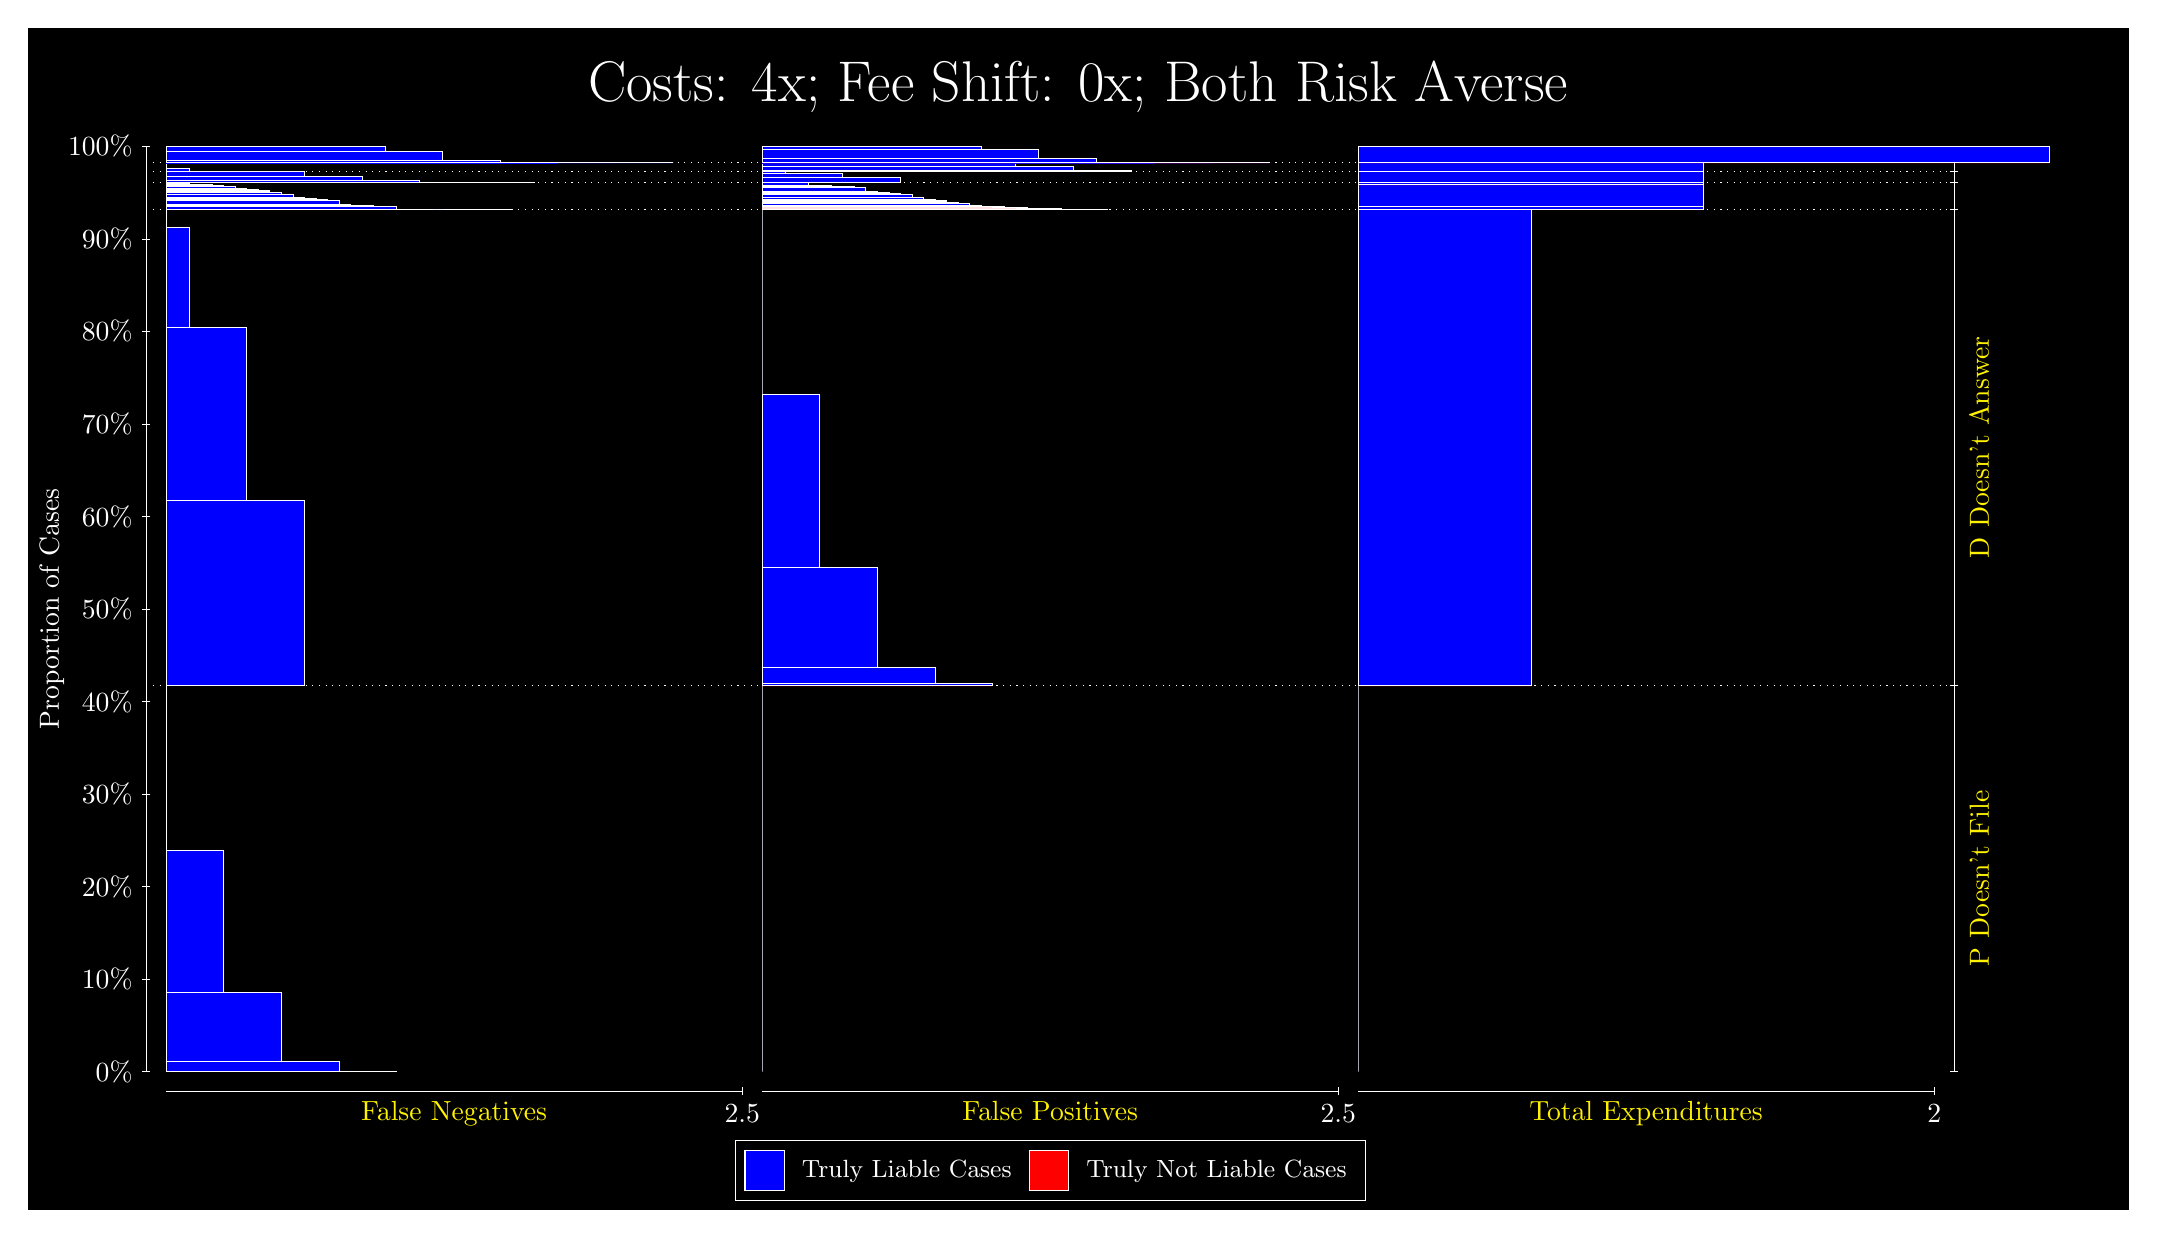
\begin{tikzpicture}
\draw[fill=black] (0,0) rectangle (26.667,15);
\draw[text=white] (0,13.5) rectangle (26.667,15) node[midway] {\huge Costs: 4x; Fee Shift: 0x; Both Risk Averse};
\draw[white, very thin] (1.5,1.75) -- (1.5,13.5);
\node[rotate=90, text=white, anchor=center] at (0.3, 7.625) {Proportion of Cases};
\draw[white, very thin] (1.45,1.75) -- (1.55,1.75);
\node[text=white, anchor=east] at (1.45, 1.75) {0\%};
\draw[white, very thin] (1.45,2.925) -- (1.55,2.925);
\node[text=white, anchor=east] at (1.45, 2.925) {10\%};
\draw[white, very thin] (1.45,4.1) -- (1.55,4.1);
\node[text=white, anchor=east] at (1.45, 4.1) {20\%};
\draw[white, very thin] (1.45,5.275) -- (1.55,5.275);
\node[text=white, anchor=east] at (1.45, 5.275) {30\%};
\draw[white, very thin] (1.45,6.45) -- (1.55,6.45);
\node[text=white, anchor=east] at (1.45, 6.45) {40\%};
\draw[white, very thin] (1.45,7.625) -- (1.55,7.625);
\node[text=white, anchor=east] at (1.45, 7.625) {50\%};
\draw[white, very thin] (1.45,8.8) -- (1.55,8.8);
\node[text=white, anchor=east] at (1.45, 8.8) {60\%};
\draw[white, very thin] (1.45,9.975) -- (1.55,9.975);
\node[text=white, anchor=east] at (1.45, 9.975) {70\%};
\draw[white, very thin] (1.45,11.15) -- (1.55,11.15);
\node[text=white, anchor=east] at (1.45, 11.15) {80\%};
\draw[white, very thin] (1.45,12.325) -- (1.55,12.325);
\node[text=white, anchor=east] at (1.45, 12.325) {90\%};
\draw[white, very thin] (1.45,13.5) -- (1.55,13.5);
\node[text=white, anchor=east] at (1.45, 13.5) {100\%};

\draw[white, very thin] (24.457,1.75) -- (24.457,13.5);
\draw[white, very thin] (24.407,1.75) -- (24.507,1.75);
\node[anchor=west] at (24.407, 1.75) {};
\draw[white, very thin] (24.407,6.651) -- (24.507,6.651);
\node[anchor=west] at (24.407, 6.651) {};
\draw[white, very thin] (24.407,12.702) -- (24.507,12.702);
\node[anchor=west] at (24.407, 12.702) {};
\draw[white, very thin] (24.407,13.045) -- (24.507,13.045);
\node[anchor=west] at (24.407, 13.045) {};
\draw[white, very thin] (24.407,13.182) -- (24.507,13.182);
\node[anchor=west] at (24.407, 13.182) {};
\draw[white, very thin] (24.407,13.293) -- (24.507,13.293);
\node[anchor=west] at (24.407, 13.293) {};
\draw[white, very thin] (24.407,13.5) -- (24.507,13.5);
\node[anchor=west] at (24.407, 13.5) {};

\draw[white, very thin, fill=blue] (1.75,1.75) rectangle (4.6775,1.7513);
\draw[white, very thin, fill=blue] (1.75,1.7513) rectangle (3.9457,1.8842);
\draw[white, very thin, fill=blue] (1.75,1.8842) rectangle (3.2138,2.7579);
\draw[white, very thin, fill=blue] (1.75,2.7579) rectangle (2.4819,4.555);
\draw[white, very thin, fill=red] (1.75,4.555) rectangle (1.75,4.555);
\draw[white, very thin, fill=blue] (1.75,4.555) rectangle (1.75,6.651);
\draw[white, very thin, fill=blue] (1.75,6.651) rectangle (3.5065,8.9994);
\draw[white, very thin, fill=blue] (1.75,8.9994) rectangle (2.7746,11.201);
\draw[white, very thin, fill=blue] (1.75,11.201) rectangle (2.0428,12.47);
\draw[white, very thin, fill=red] (1.75,12.47) rectangle (1.75,12.47);
\draw[white, very thin, fill=blue] (1.75,12.47) rectangle (1.75,12.702);
\draw[white, very thin, fill=blue] (1.75,12.702) rectangle (6.1413,12.702);
\draw[white, very thin, fill=blue] (1.75,12.702) rectangle (5.8486,12.702);
\draw[white, very thin, fill=blue] (1.75,12.702) rectangle (5.5558,12.702);
\draw[white, very thin, fill=blue] (1.75,12.702) rectangle (5.4094,12.704);
\draw[white, very thin, fill=blue] (1.75,12.704) rectangle (5.2631,12.704);
\draw[white, very thin, fill=blue] (1.75,12.704) rectangle (5.1167,12.705);
\draw[white, very thin, fill=blue] (1.75,12.705) rectangle (4.9703,12.705);
\draw[white, very thin, fill=blue] (1.75,12.705) rectangle (4.8239,12.705);
\draw[white, very thin, fill=blue] (1.75,12.705) rectangle (4.6775,12.738);
\draw[white, very thin, fill=blue] (1.75,12.738) rectangle (4.5312,12.739);
\draw[white, very thin, fill=blue] (1.75,12.739) rectangle (4.3848,12.739);
\draw[white, very thin, fill=blue] (1.75,12.739) rectangle (4.3848,12.752);
\draw[white, very thin, fill=blue] (1.75,12.752) rectangle (4.2384,12.753);
\draw[white, very thin, fill=blue] (1.75,12.753) rectangle (4.092,12.769);
\draw[white, very thin, fill=blue] (1.75,12.769) rectangle (4.092,12.769);
\draw[white, very thin, fill=blue] (1.75,12.769) rectangle (3.9457,12.814);
\draw[white, very thin, fill=blue] (1.75,12.814) rectangle (3.7993,12.825);
\draw[white, very thin, fill=blue] (1.75,12.825) rectangle (3.6529,12.826);
\draw[white, very thin, fill=blue] (1.75,12.826) rectangle (3.6529,12.844);
\draw[white, very thin, fill=blue] (1.75,12.844) rectangle (3.5065,12.859);
\draw[white, very thin, fill=blue] (1.75,12.859) rectangle (3.3602,12.889);
\draw[white, very thin, fill=blue] (1.75,12.889) rectangle (3.3602,12.89);
\draw[white, very thin, fill=blue] (1.75,12.89) rectangle (3.2138,12.922);
\draw[white, very thin, fill=blue] (1.75,12.922) rectangle (3.0674,12.928);
\draw[white, very thin, fill=blue] (1.75,12.928) rectangle (3.0674,12.936);
\draw[white, very thin, fill=blue] (1.75,12.936) rectangle (2.921,12.943);
\draw[white, very thin, fill=blue] (1.75,12.943) rectangle (2.921,12.955);
\draw[white, very thin, fill=blue] (1.75,12.955) rectangle (2.7746,12.973);
\draw[white, very thin, fill=blue] (1.75,12.973) rectangle (2.6283,12.991);
\draw[white, very thin, fill=blue] (1.75,12.991) rectangle (2.6283,12.994);
\draw[white, very thin, fill=blue] (1.75,12.994) rectangle (2.4819,13.007);
\draw[white, very thin, fill=blue] (1.75,13.007) rectangle (2.3355,13.009);
\draw[white, very thin, fill=blue] (1.75,13.009) rectangle (2.3355,13.013);
\draw[white, very thin, fill=blue] (1.75,13.013) rectangle (2.1891,13.021);
\draw[white, very thin, fill=blue] (1.75,13.021) rectangle (2.0428,13.027);
\draw[white, very thin, fill=blue] (1.75,13.027) rectangle (1.8964,13.031);
\draw[white, very thin, fill=red] (1.75,13.031) rectangle (1.75,13.031);
\draw[white, very thin, fill=blue] (1.75,13.031) rectangle (1.75,13.045);
\draw[white, very thin, fill=blue] (1.75,13.045) rectangle (6.4341,13.045);
\draw[white, very thin, fill=blue] (1.75,13.045) rectangle (5.7022,13.045);
\draw[white, very thin, fill=blue] (1.75,13.045) rectangle (4.9703,13.063);
\draw[white, very thin, fill=blue] (1.75,13.063) rectangle (4.2384,13.122);
\draw[white, very thin, fill=blue] (1.75,13.122) rectangle (3.5065,13.182);
\draw[white, very thin, fill=red] (1.75,13.182) rectangle (1.75,13.182);
\draw[white, very thin, fill=blue] (1.75,13.182) rectangle (3.5065,13.182);
\draw[white, very thin, fill=blue] (1.75,13.182) rectangle (2.7746,13.187);
\draw[white, very thin, fill=blue] (1.75,13.187) rectangle (2.0428,13.226);
\draw[white, very thin, fill=red] (1.75,13.226) rectangle (1.75,13.226);
\draw[white, very thin, fill=blue] (1.75,13.226) rectangle (1.75,13.293);
\draw[white, very thin, fill=blue] (1.75,13.293) rectangle (8.1906,13.293);
\draw[white, very thin, fill=blue] (1.75,13.293) rectangle (7.4587,13.293);
\draw[white, very thin, fill=blue] (1.75,13.293) rectangle (6.7268,13.294);
\draw[white, very thin, fill=blue] (1.75,13.294) rectangle (5.9949,13.325);
\draw[white, very thin, fill=blue] (1.75,13.325) rectangle (5.2631,13.441);
\draw[white, very thin, fill=blue] (1.75,13.441) rectangle (4.5312,13.495);
\draw[white, very thin, fill=blue] (1.75,13.495) rectangle (3.7993,13.5);
\draw[white, very thin, fill=blue] (1.75,13.5) rectangle (3.0674,13.5);
\draw[white, very thin, fill=blue] (1.75,13.5) rectangle (2.3355,13.5);
\draw[white, very thin, fill=red] (1.75,13.5) rectangle (1.75,13.5);
\draw[white, very thin, fill=red] (9.3189,1.75) rectangle (9.3189,1.75);
\draw[white, very thin, fill=blue] (9.3189,1.75) rectangle (9.3189,6.651);
\draw[white, very thin, fill=red] (9.3189,6.651) rectangle (12.246,6.651);
\draw[white, very thin, fill=blue] (9.3189,6.651) rectangle (12.246,6.683);
\draw[white, very thin, fill=blue] (9.3189,6.683) rectangle (11.515,6.8828);
\draw[white, very thin, fill=blue] (9.3189,6.8828) rectangle (10.783,8.1521);
\draw[white, very thin, fill=blue] (9.3189,8.1521) rectangle (10.051,10.353);
\draw[white, very thin, fill=blue] (9.3189,10.353) rectangle (9.3189,12.702);
\draw[white, very thin, fill=red] (9.3189,12.702) rectangle (13.71,12.702);
\draw[white, very thin, fill=blue] (9.3189,12.702) rectangle (13.71,12.704);
\draw[white, very thin, fill=red] (9.3189,12.704) rectangle (13.417,12.704);
\draw[white, very thin, fill=blue] (9.3189,12.704) rectangle (13.417,12.705);
\draw[white, very thin, fill=red] (9.3189,12.705) rectangle (13.125,12.705);
\draw[white, very thin, fill=blue] (9.3189,12.705) rectangle (13.125,12.709);
\draw[white, very thin, fill=blue] (9.3189,12.709) rectangle (12.978,12.712);
\draw[white, very thin, fill=red] (9.3189,12.712) rectangle (12.832,12.712);
\draw[white, very thin, fill=blue] (9.3189,12.712) rectangle (12.832,12.716);
\draw[white, very thin, fill=blue] (9.3189,12.716) rectangle (12.686,12.72);
\draw[white, very thin, fill=red] (9.3189,12.72) rectangle (12.539,12.72);
\draw[white, very thin, fill=blue] (9.3189,12.72) rectangle (12.539,12.725);
\draw[white, very thin, fill=blue] (9.3189,12.725) rectangle (12.393,12.734);
\draw[white, very thin, fill=red] (9.3189,12.734) rectangle (12.246,12.734);
\draw[white, very thin, fill=blue] (9.3189,12.734) rectangle (12.246,12.739);
\draw[white, very thin, fill=blue] (9.3189,12.739) rectangle (12.1,12.752);
\draw[white, very thin, fill=red] (9.3189,12.752) rectangle (11.954,12.752);
\draw[white, very thin, fill=blue] (9.3189,12.752) rectangle (11.954,12.773);
\draw[white, very thin, fill=blue] (9.3189,12.773) rectangle (11.807,12.792);
\draw[white, very thin, fill=red] (9.3189,12.792) rectangle (11.661,12.792);
\draw[white, very thin, fill=blue] (9.3189,12.792) rectangle (11.661,12.804);
\draw[white, very thin, fill=blue] (9.3189,12.804) rectangle (11.661,12.811);
\draw[white, very thin, fill=blue] (9.3189,12.811) rectangle (11.515,12.825);
\draw[white, very thin, fill=red] (9.3189,12.825) rectangle (11.368,12.825);
\draw[white, very thin, fill=blue] (9.3189,12.825) rectangle (11.368,12.857);
\draw[white, very thin, fill=blue] (9.3189,12.857) rectangle (11.222,12.888);
\draw[white, very thin, fill=blue] (9.3189,12.888) rectangle (11.075,12.903);
\draw[white, very thin, fill=blue] (9.3189,12.903) rectangle (10.929,12.921);
\draw[white, very thin, fill=blue] (9.3189,12.921) rectangle (10.929,12.922);
\draw[white, very thin, fill=blue] (9.3189,12.922) rectangle (10.783,12.933);
\draw[white, very thin, fill=blue] (9.3189,12.933) rectangle (10.636,12.978);
\draw[white, very thin, fill=blue] (9.3189,12.978) rectangle (10.49,12.994);
\draw[white, very thin, fill=blue] (9.3189,12.994) rectangle (10.344,12.995);
\draw[white, very thin, fill=blue] (9.3189,12.995) rectangle (10.197,13.008);
\draw[white, very thin, fill=blue] (9.3189,13.008) rectangle (10.197,13.008);
\draw[white, very thin, fill=blue] (9.3189,13.008) rectangle (10.051,13.009);
\draw[white, very thin, fill=blue] (9.3189,13.009) rectangle (9.9044,13.041);
\draw[white, very thin, fill=blue] (9.3189,13.041) rectangle (9.758,13.042);
\draw[white, very thin, fill=blue] (9.3189,13.042) rectangle (9.6116,13.042);
\draw[white, very thin, fill=blue] (9.3189,13.042) rectangle (9.4652,13.043);
\draw[white, very thin, fill=blue] (9.3189,13.043) rectangle (9.3189,13.045);
\draw[white, very thin, fill=red] (9.3189,13.045) rectangle (11.075,13.045);
\draw[white, very thin, fill=blue] (9.3189,13.045) rectangle (11.075,13.105);
\draw[white, very thin, fill=blue] (9.3189,13.105) rectangle (10.344,13.164);
\draw[white, very thin, fill=blue] (9.3189,13.164) rectangle (9.6116,13.182);
\draw[white, very thin, fill=blue] (9.3189,13.182) rectangle (9.3189,13.182);
\draw[white, very thin, fill=red] (9.3189,13.182) rectangle (14.003,13.182);
\draw[white, very thin, fill=blue] (9.3189,13.182) rectangle (14.003,13.197);
\draw[white, very thin, fill=blue] (9.3189,13.197) rectangle (13.271,13.249);
\draw[white, very thin, fill=blue] (9.3189,13.249) rectangle (12.539,13.289);
\draw[white, very thin, fill=blue] (9.3189,13.289) rectangle (11.807,13.293);
\draw[white, very thin, fill=blue] (9.3189,13.293) rectangle (11.075,13.293);
\draw[white, very thin, fill=red] (9.3189,13.293) rectangle (15.759,13.293);
\draw[white, very thin, fill=blue] (9.3189,13.293) rectangle (15.759,13.293);
\draw[white, very thin, fill=blue] (9.3189,13.293) rectangle (15.028,13.293);
\draw[white, very thin, fill=red] (9.3189,13.293) rectangle (15.028,13.293);
\draw[white, very thin, fill=blue] (9.3189,13.293) rectangle (15.028,13.293);
\draw[white, very thin, fill=blue] (9.3189,13.293) rectangle (14.296,13.294);
\draw[white, very thin, fill=red] (9.3189,13.294) rectangle (14.296,13.294);
\draw[white, very thin, fill=blue] (9.3189,13.294) rectangle (14.296,13.299);
\draw[white, very thin, fill=blue] (9.3189,13.299) rectangle (13.564,13.299);
\draw[white, very thin, fill=red] (9.3189,13.299) rectangle (13.564,13.299);
\draw[white, very thin, fill=blue] (9.3189,13.299) rectangle (13.564,13.352);
\draw[white, very thin, fill=blue] (9.3189,13.352) rectangle (12.832,13.352);
\draw[white, very thin, fill=red] (9.3189,13.352) rectangle (12.832,13.352);
\draw[white, very thin, fill=blue] (9.3189,13.352) rectangle (12.832,13.468);
\draw[white, very thin, fill=blue] (9.3189,13.468) rectangle (12.1,13.499);
\draw[white, very thin, fill=blue] (9.3189,13.499) rectangle (11.368,13.5);
\draw[white, very thin, fill=blue] (9.3189,13.5) rectangle (10.636,13.5);
\draw[white, very thin, fill=blue] (9.3189,13.5) rectangle (9.9044,13.5);
\draw[white, very thin, fill=red] (16.888,1.75) rectangle (16.888,1.75);
\draw[white, very thin, fill=blue] (16.888,1.75) rectangle (16.888,6.651);
\draw[white, very thin, fill=red] (16.888,6.651) rectangle (19.083,6.651);
\draw[white, very thin, fill=blue] (16.888,6.651) rectangle (19.083,12.702);
\draw[white, very thin, fill=red] (16.888,12.702) rectangle (21.279,12.702);
\draw[white, very thin, fill=blue] (16.888,12.702) rectangle (21.279,12.742);
\draw[white, very thin, fill=red] (16.888,12.742) rectangle (21.279,12.742);
\draw[white, very thin, fill=blue] (16.888,12.742) rectangle (21.279,13.015);
\draw[white, very thin, fill=red] (16.888,13.015) rectangle (21.279,13.015);
\draw[white, very thin, fill=blue] (16.888,13.015) rectangle (21.279,13.045);
\draw[white, very thin, fill=red] (16.888,13.045) rectangle (21.279,13.045);
\draw[white, very thin, fill=blue] (16.888,13.045) rectangle (21.279,13.182);
\draw[white, very thin, fill=red] (16.888,13.182) rectangle (21.279,13.182);
\draw[white, very thin, fill=blue] (16.888,13.182) rectangle (21.279,13.293);
\draw[white, very thin, fill=red] (16.888,13.293) rectangle (25.67,13.293);
\draw[white, very thin, fill=blue] (16.888,13.293) rectangle (25.67,13.295);
\draw[white, very thin, fill=red] (16.888,13.295) rectangle (25.67,13.295);
\draw[white, very thin, fill=blue] (16.888,13.295) rectangle (25.67,13.5);
\draw[white, dotted] (1.5,6.651) -- (24.457,6.651);
\draw[white, dotted] (1.5,12.702) -- (24.457,12.702);
\draw[white, dotted] (1.5,13.045) -- (24.457,13.045);
\draw[white, dotted] (1.5,13.182) -- (24.457,13.182);
\draw[white, dotted] (1.5,13.293) -- (24.457,13.293);
\draw[white, very thin] (1.75,1.5) -- (9.0689,1.5);
\node[text=yellow, anchor=north] at (5.4094, 1.5) {False Negatives};
\draw[white, very thin] (9.0689,1.45) -- (9.0689,1.55);
\node[text=white, anchor=north] at (9.0689, 1.45) {2.5};

\draw[white, very thin] (9.3189,1.5) -- (16.638,1.5);
\node[text=yellow, anchor=north] at (12.978, 1.5) {False Positives};
\draw[white, very thin] (16.638,1.45) -- (16.638,1.55);
\node[text=white, anchor=north] at (16.638, 1.45) {2.5};

\draw[white, very thin] (16.888,1.5) -- (24.207,1.5);
\node[text=yellow, anchor=north] at (20.547, 1.5) {Total Expenditures};
\draw[white, very thin] (24.207,1.45) -- (24.207,1.55);
\node[text=white, anchor=north] at (24.207, 1.45) {2};

\node[text=yellow, centered, rotate=90] at (24.777, 4.2005) {P Doesn't File};
\node[text=yellow, centered, rotate=90] at (24.777, 9.6765) {D Doesn't Answer};





\draw (12.978300999999998,1.5) node[draw=none] (baseCoordinate) {};
\begin{scope}[align=center]
        \matrix[scale=0.5, draw=white, below=0.5cm of baseCoordinate, nodes={draw}, column sep=0.1cm]{
            \node[rectangle, draw, minimum width=0.5cm, minimum height=0.5cm, fill=blue] {}; &
            \node[draw=none, font=\small, text=white] (B) {Truly Liable Cases}; &
            \node[rectangle, draw, minimum width=0.5cm, minimum height=0.5cm, fill=red] {}; &
            \node[draw=none, font=\small, text=white] (B) {Truly Not Liable Cases}; \\
            };
\end{scope}

\end{tikzpicture}
\end{document}